\documentclass[10pt]{beamer}
\usetheme[
%%% option passed to the outer theme
%    progressstyle=fixedCircCnt,   % fixedCircCnt, movingCircCnt (moving is deault)
  ]{Feather}
  
% If you want to change the colors of the various elements in the theme, edit and uncomment the following lines

% Change the bar colors:
\setbeamercolor{Feather}{fg=black!20,bg=black}

% Change the color of the structural elements:
\setbeamercolor{structure}{fg=black}

% Change the frame title text color:
%\setbeamercolor{frametitle}{fg=blue}

% Change the normal text color background:
%\setbeamercolor{normal text}{fg=black,bg=gray!10}

%-------------------------------------------------------
% INCLUDE PACKAGES
%-------------------------------------------------------

\usepackage[utf8]{inputenc}
\usepackage[polish]{babel}
\usepackage{polski}
\usepackage[T1]{fontenc}
\usepackage{helvet}
\usepackage{booktabs}
\usepackage{array}
\usepackage{setspace}
\usepackage{graphicx}
\usepackage{caption}


%-------------------------------------------------------
% DEFFINING AND REDEFINING COMMANDS
%-------------------------------------------------------
\DeclareCaptionLabelSeparator{kropka}{. }
\setbeamertemplate{caption}[numbered]
\captionsetup[figure]{labelformat=simple, labelsep=kropka}
\captionsetup[table]{labelformat=simple, labelsep=kropka}
\addto\captionspolish{\renewcommand{\tablename}{Tabela}}

\newcolumntype{k}[1]{>{\centering\arraybackslash}m{#1}}

% colored hyperlinks
\newcommand{\chref}[2]{
  \href{#1}{{\usebeamercolor[bg]{Feather}#2}}
}

%-------------------------------------------------------
% INFORMATION IN THE TITLE PAGE
%-------------------------------------------------------

\title[Polska szkoła sztucznej inteligencji – zbiory przybliżone] % [] is optional - is placed on the bottom of the sidebar on every slide
{ % is placed on the title page
      \textbf{Zbiory przybliżone}
}

\subtitle[]
{
      \textbf{Polska szkoła sztucznej inteligencji}
}

\author[Jan Gromko]
{
\textbf{Jan Gromko}
}

\institute[SKN Math4You WI PB]
{
      Studenckie Koło Naukowe Math4You\\
      Wydział Informatyki Politechniki Białostockiej
}

\date{22 kwietnia 2017 r.}


\begin{document}


{\1% wybór pliku na tło
\begin{frame}[plain,noframenumbering]
  \titlepage
\end{frame}}


\begin{frame}{Plan referatu}{}
\tableofcontents
\end{frame}

%-------------------------------------------------------
\section{Wprowadzenie}
%-------------------------------------------------------
\subsection{Czym są zbiory przybliżone – historia i idea}
\begin{frame}{Historia i idea}
\begin{spacing}{1.5}
\begin{itemize}
\item Teoria zaproponowana w 1982 r. przez prof. Zdzisława Pawlaka.
\item Wprowadzona jako nowe matematyczne podejście do pojęć nieostrych i metoda analizy danych.
\end{itemize}
\end{spacing}

\end{frame}

%-------------------------------------------------------
\subsection{Podstawowe pojęcia}
\begin{frame}{Podstawy}
\begin{spacing}{1.5}
\begin{itemize}
\item Zbiory przybliżone oparte są o logikę trójwartościową;
\item zbiór przybliżony jest zbiorem niedefiniowalnym -- nie można go jednoznacznie scharakteryzować na podstawie własności jego elementów.
\end{itemize}

\end{spacing}
\end{frame}


\begin{frame}{Przykład}
\begin{center}
\begin{table}
\begin{tabular}{|k{1.2cm}|k{1.8cm}|k{1.8cm}|k{2.2cm}|k{1.4cm}|@{}m{0pt}@{}}
\hline
\textit{Pacjent} & \textit{Ból głowy} & \textit{Ból mięśni} & \textit{Temperatura} &  \textit{Grypa} &\\[1ex]
\hline
1 & nie & tak & podwyższona & tak &\\[1ex]
2 & tak & nie & podwyższona & tak &\\[1ex]
3 & tak & tak & wysoka & tak &\\[1ex]
4 & nie & tak & normalna & nie &\\[1ex]
5 & tak & nie & podwyższona & nie &\\[1ex]
6 & nie & nie & wysoka & tak &\\[1ex]
\hline
\end{tabular}
\caption{Tablica decyzyjna przykładowego zbioru.}
\end{table}
\end{center}
\end{frame}




\begin{frame}
\frametitle{Podstawowe pojęcia}
\begin{spacing}{1.7}
\begin{flushleft}
$S = (U, A, V, f)$ -- system informacyjny\\
$U$ -- zbiór obiektów (\textit{uniwersum})\\
$A$ -- zbiór atrybutów\\
$V = \bigcup\limits_{a \in A} V_{a}$ -- zbiór wszystkich możliwych wartości atrybutów\\
$V_{a}$ -- dziedzina atrybutu $a \in A$\\
$f : U \times A \rightarrow V$ -- funkcja informacyjna\\
\end{flushleft}
\end{spacing}
\end{frame}


\begin{frame}
\frametitle{Podstawowe pojęcia}
\begin{spacing}{1.7}
\begin{flushleft}
$DT = (U, C, D, V, f)$ -- tablica decyzyjna\\
$C$ -- zbiór atrybutów warunkowych\\
$D$ -- zbiór atrybutów decyzyjnych\\
$A = C \cup D$ -- zbiór atrybutów\\
\end{flushleft}
\end{spacing}
\end{frame}


\begin{frame}
\frametitle{Podstawowe pojęcia}
\begin{spacing}{1.7}
\begin{flushleft}
$U$ -- pacjenci\\
$C = \lbrace$\textit{ból głowy, ból mięśni, temperatura}$\rbrace$\\
$D$ -- \textit{grypa}\\
\end{flushleft}
\end{spacing}
\end{frame}





\begin{frame}{Reguły decyzyjne}
\begin{spacing}{1.5}
\textbf{Problem:}\\
Znaleźć zależność między występowaniem/niewystępowaniem grypy a symptomami występującymi u pacjentów, czyli znaleźć zależność między atrybutem decyzyjnym a wartościami atrybutów warunkowych, opisujących poszczególne obiekty.
\end{spacing}
\end{frame}


\begin{frame}{Sprzeczności w zbiorze}
\renewcommand{\arraystretch}{1}
\begin{center}
\begin{table}
\begin{tabular}{|k{1.2cm}|k{1.8cm}|k{1.8cm}|k{2.2cm}|k{1.4cm}|@{}m{0pt}@{}}
\hline
\textit{Pacjent} & \textit{Ból głowy} & \textit{Ból mięśni} & \textit{Temperatura} &  \textit{Grypa} &\\[1ex]
\hline
2 & tak & nie & podwyższona & tak &\\[1ex]
5 & tak & nie & podwyższona & nie &\\[1ex]
\hline
\end{tabular}
\caption{Sprzeczne informacje w zbiorze -- przypadki, których nie można jednoznacznie sklasyfikować.}
\end{table}
\end{center}
\end{frame}


\begin{frame}{Podstawowe pojęcia}
\begin{block}{Relacja nierozróżnialności}
Relację nierozróżnialności zdefiniowana jest jako
$$I(B)=\lbrace (x,y) \in U \times U: \forall a \in B~~f(a,x)=f(a,y) \rbrace,$$
gdzie $B \subseteq A$.\\
$\newline$
Jeśli $(x, y) \in I(B)$, wówczas obiekty $x$ i $y$ są nierozróżnialne ze~względu na podzbiór atrybutów $B$.
\end{block}
\end{frame}


\begin{frame}{Przykład -- analiza danych}
\begin{spacing}{1.5}
\textbf{W oparciu o posiadane dane, można stwierdzić, że:}\\
\begin{itemize}
\item $\lbrace 1,3,6 \rbrace$ to zbiór przypadków, które (na podstawie atrybutów warunkowych) możemy \textit{jednoznacznie} zaklasyfikować do grupy pacjentów chorych na grypę;
\item $\lbrace 1,2,3,5,6 \rbrace$ to zbiór przypadków, które \textit{mogą} być zakwalifikowanie jako pacjenci chorzy na grypę;
\item $\lbrace 2,5 \rbrace$ to zbiór przypadków, które nie mogą być jednoznacznie zaklasyfikowane jako pacjenci, którzy są lub nie są chorzy na~grypę.
\end{itemize}
\end{spacing}
\end{frame}


\begin{frame}{Podstawowe pojęcia}
\begin{spacing}{1.2}
\begin{block}{Dolne przybliżenie}
Wszystkie te elementy, które można jednoznacznie zaklasyfikować do danego zbioru, według posiadanej wiedzy na ich temat.
\end{block}
\begin{block}{Górne przybliżenie}
Wszystkie te elementy, których przynależności do danego zbioru nie można wykluczyć.
\end{block}
\end{spacing}
\end{frame}


\begin{frame}{Podstawowe pojęcia}
\begin{center}
\begin{figure}
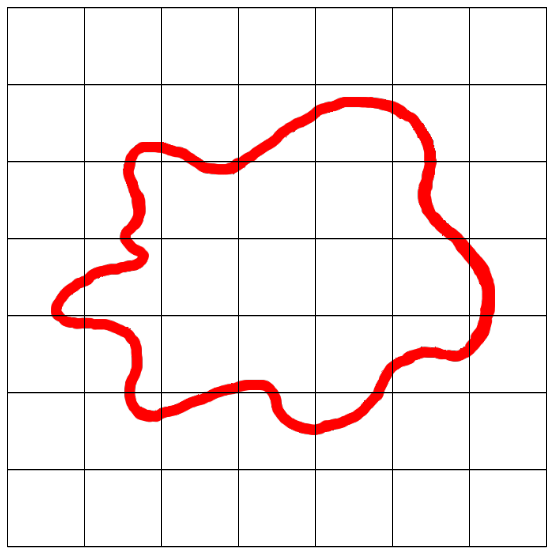
\includegraphics[width=0.55\textwidth]{Grafiki/plama.png}
\caption{Przykładowy zbiór.}
\end{figure}
\end{center}
\end{frame}


\begin{frame}{Dolne przybliżenie}
\begin{center}
\begin{figure}
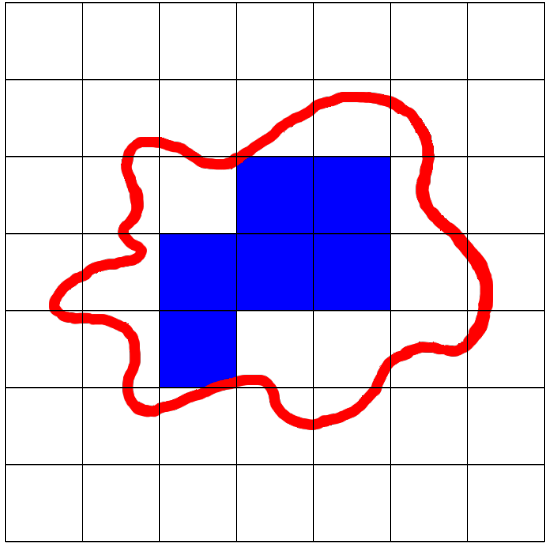
\includegraphics[width=0.55\textwidth]{Grafiki/dolne_przyblizenie.png}
\caption{Dolne przybliżenie zbioru.}
\end{figure}

\end{center}
\end{frame}


\begin{frame}{Obszar brzegowy}
\begin{center}
\begin{figure}
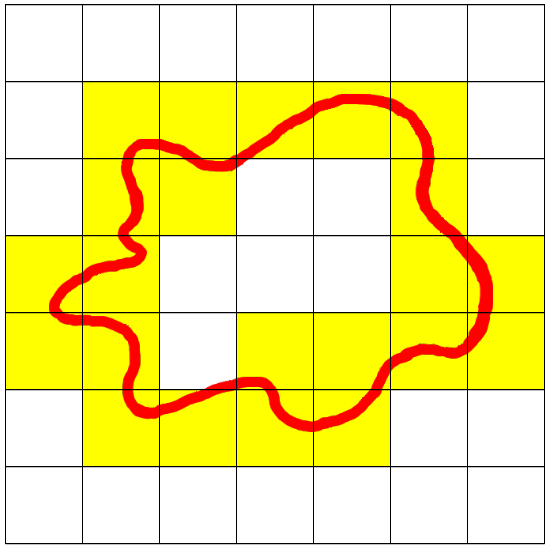
\includegraphics[width=0.55\textwidth]{Grafiki/obszar_brzegowy.png}
\caption{Obszar brzegowy zbioru.}
\end{figure}

\end{center}
\end{frame}


\begin{frame}{Górne przybliżenie}
\begin{center}
\begin{figure}
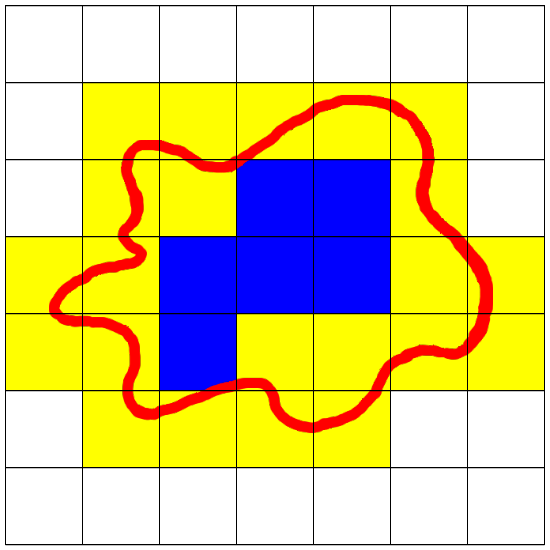
\includegraphics[width=0.55\textwidth]{Grafiki/gorne_przyblizenie.png}
\caption{Górne przybliżenie zbioru.}
\end{figure}
\end{center}
\end{frame}


\section{Problem redukcji}

\subsection{Istota problemu redukcji}
\begin{frame}{Redukcja}
\begin{spacing}{1.5}
\textbf{Czy można zredukować zbiór pod~względem atrybutów w~ten~sposób, by~zachowana była rozróżnialność elementów z~oryginalnego zbioru?}
\end{spacing}
\end{frame}


\begin{frame}{Macierz rozróżnialności}
\renewcommand{\arraystretch}{1}
\begin{center}
\begin{table}
\begin{tabular}{|k{1cm}|k{1cm}|k{1cm}|k{1cm}|k{1cm}|k{1cm}|k{1cm}|@{}m{0pt}@{}}
\hline
& 1 & 2 & 3 & 4 & 5 & 6&\\[1ex]
\hline
1 & $\emptyset$ & -- & -- & -- & -- & -- &\\[1ex]
\hline
2 & $\emptyset$ & $\emptyset$ & -- & -- & -- & -- &\\[1ex]
\hline
3 & $\emptyset$ & $\emptyset$ & $\emptyset$ & -- & -- & -- &\\[1ex]
\hline
4 & t & g, m, t & g, t & $\emptyset$ & -- & -- &\\[1ex]
\hline
5 & g, m & $\emptyset$ & m, t & $\emptyset$ & $\emptyset$ & -- &\\[1ex]
\hline
6 &$\emptyset$ & $\emptyset$ & $\emptyset$ & m, t & g, t & $\emptyset$ &\\[1ex]
\hline
\end{tabular}
\caption{Macierz rozróżnialności.}
\end{table}

\end{center}

\begin{flushleft}
\textit{g} -- ból głowy; 
\textit{m} -- ból mięśni; 
\textit{t} -- temperatura
\end{flushleft}

\end{frame}


\begin{frame}{Tworzenie macierzy rozróżnialności}
\renewcommand{\arraystretch}{1}
\begin{center}

\begin{table}
\begin{tabular}{|k{1.2cm}|k{1.8cm}|k{1.8cm}|k{2.2cm}|k{1.4cm}|@{}m{0pt}@{}}
\hline
\textit{Pacjent} & \textit{Ból głowy} & \textit{Ból mięśni} & \textit{Temperatura} &  \textit{Grypa} &\\[1ex]
\hline
1 & nie & tak & podwyższona & tak &\\[1ex]
4 & nie & tak & normalna & nie &\\[1ex]
\hline
\end{tabular}
\caption{Fragment tablicy decyzyjnej.}
\end{table}

\begin{table}
\begin{tabular}{|k{1cm}|k{1cm}|k{1cm}|k{1cm}|k{1cm}|k{1cm}|k{1cm}|@{}m{0pt}@{}}
\hline
& 1 & 2 & 3 & 4 & 5 & 6 & \\[1ex]
\hline
4 & t & ? & ? & $\emptyset$ & -- & -- &\\[1ex]
\hline
\end{tabular}
\caption{Fragment macierzy rozróżnialności.}
\end{table}

\end{center}

\end{frame}


\begin{frame}{Tworzenie macierzy rozróżnialności}
\renewcommand{\arraystretch}{1}
\begin{center}

\begin{table}
\begin{tabular}{|k{1.2cm}|k{1.8cm}|k{1.8cm}|k{2.2cm}|k{1.4cm}|@{}m{0pt}@{}}
\hline
\textit{Pacjent} & \textit{Ból głowy} & \textit{Ból mięśni} & \textit{Temperatura} &  \textit{Grypa} &\\[1ex]
\hline
2 & tak & nie & podwyższona & tak &\\[1ex]
4 & nie & tak & normalna & nie &\\[1ex]
\hline
\end{tabular}
\caption{Fragment tablicy decyzyjnej.}
\end{table}

\begin{table}
\begin{tabular}{|k{1cm}|k{1cm}|k{1cm}|k{1cm}|k{1cm}|k{1cm}|k{1cm}|@{}m{0pt}@{}}
\hline
& 1 & 2 & 3 & 4 & 5 & 6 & \\[1ex]
\hline
4 & t & g, m, t & ? & $\emptyset$ & -- & -- &\\[1ex]
\hline
\end{tabular}
\caption{Fragment macierzy rozróżnialności.}
\end{table}

\end{center}

\end{frame}


\begin{frame}{Tworzenie macierzy rozróżnialności}
\renewcommand{\arraystretch}{1}
\begin{center}

\begin{table}
\begin{tabular}{|k{1.2cm}|k{1.8cm}|k{1.8cm}|k{2.2cm}|k{1.4cm}|@{}m{0pt}@{}}
\hline
\textit{Pacjent} & \textit{Ból głowy} & \textit{Ból mięśni} & \textit{Temperatura} &  \textit{Grypa} &\\[1ex]
\hline
3 & tak & tak & wysoka & tak &\\[1ex]
4 & nie & tak & normalna & nie &\\[1ex]
\hline
\end{tabular}
\caption{Fragment tablicy decyzyjnej.}
\end{table}

\begin{table}
\begin{tabular}{|k{1cm}|k{1cm}|k{1cm}|k{1cm}|k{1cm}|k{1cm}|k{1cm}|@{}m{0pt}@{}}
\hline
& 1 & 2 & 3 & 4 & 5 & 6 & \\[1ex]
\hline
4 & t & g, m, t & g, t & $\emptyset$ & -- & -- &\\[1ex]
\hline
\end{tabular}
\caption{Fragment macierzy rozróżnialności.}
\end{table}

\end{center}

\end{frame}



\begin{frame}{Macierz rozróżnialności -- oryginalny zbiór}
\renewcommand{\arraystretch}{1}
\begin{center}
\begin{table}
\begin{tabular}{|k{1cm}|k{1cm}|k{1cm}|k{1cm}|k{1cm}|k{1cm}|k{1cm}|@{}m{0pt}@{}}
\hline
& 1 & 2 & 3 & 4 & 5 & 6&\\[1ex]
\hline
1 & $\emptyset$ & -- & -- & -- & -- & -- &\\[1ex]
\hline
2 & $\emptyset$ & $\emptyset$ & -- & -- & -- & -- &\\[1ex]
\hline
3 & $\emptyset$ & $\emptyset$ & $\emptyset$ & -- & -- & -- &\\[1ex]
\hline
4 & t & g, m, t & g, t & $\emptyset$ & -- & -- &\\[1ex]
\hline
5 & g, m & $\emptyset$ & m, t & $\emptyset$ & $\emptyset$ & -- &\\[1ex]
\hline
6 &$\emptyset$ & $\emptyset$ & $\emptyset$ & m, t & g, t & $\emptyset$ &\\[1ex]
\hline
\end{tabular}
\caption{Macierz rozróżnialności.}
\end{table}

\end{center}

\end{frame}



\begin{frame}{Macierz rozróżnialności -- redukcja}
\renewcommand{\arraystretch}{1}
\begin{center}
\begin{table}
\begin{tabular}{|k{1cm}|k{1cm}|k{1cm}|k{1cm}|k{1cm}|k{1cm}|k{1cm}|@{}m{0pt}@{}}
\hline
& 1 & 2 & 3 & 4 & 5 & 6 &\\[1ex]
\hline
1 & $\emptyset$ & -- & -- & -- & -- & --&\\[1ex]
\hline
2 & $\emptyset$ & $\emptyset$ & -- & -- & -- & --&\\[1ex]
\hline
3 & $\emptyset$ & $\emptyset$ & $\emptyset$ & -- & -- & --&\\[1ex]
\hline
4 & t & g, t & g, t & $\emptyset$ & -- & --&\\[1ex]
\hline
5 & g & $\emptyset$ & t & $\emptyset$ & $\emptyset$ & --&\\[1ex]
\hline
6 &$\emptyset$ & $\emptyset$ & $\emptyset$ & t & g, t & $\emptyset$&\\[1ex]
\hline
\end{tabular}
\caption{Macierz rozróżnialności po redukcji.}
\end{table}

\end{center}

\end{frame}


\subsection{Prosty algorytm redukcji}

\subsection{Problem złożoności wyznaczania reduktów}

\subsection{Przybliżone metody wyznaczania reduktu}




\section{Znaczenie zbiorów przybliżonych}
\subsection{Możliwości i zalety}
\begin{frame}{Możliwości}
\begin{spacing}{1.5}
\begin{itemize}
\item Szukanie zależności między danymi,
\item redukcja zbiorów danych,
\item określenie wagi danych,
\item generowanie reguł decyzyjnych.
\end{itemize}
\end{spacing}
\end{frame}



\begin{frame}{Zalety}
\begin{spacing}{1.5}
\begin{itemize}
\item Teoria ZP nie wymaga założeń na temat danych,\\takich jak prawdopodobieństwo czy rozmytość,
\item szybkie algorytmy analizy danych,
\item łatwa interpretacja wyników,
\item matematyczna prostota.
\end{itemize}
\end{spacing}
\end{frame}



\subsection{Zastosowania}
\begin{frame}{Zastosowania}
\begin{spacing}{1.5}
\begin{itemize}
\item Medycyna,
\item farmakologia,
\item bankowość,
\item lingwistyka,
\item rozpoznawanie mowy,
\item ochrona środowiska,
\item bazy danych.
\end{itemize}
\end{spacing}
\end{frame}


\begin{frame}{Zastosowania -- przykład}
\begin{spacing}{1.5}
Ograniczenie liczby badań medycznych do jedynie tych,\\które są naprawdę konieczne do rozpoznania choroby.

\begin{itemize}
\item Zmniejszenie ryzyka powikłań u pacjenta,
\item zmniejszenie kosztów badań.
\end{itemize}
\end{spacing}
\end{frame}



% KONIEC – BIBLIOGRAFIA I SLAJD KOŃCOWY NA PYTANIA

\begin{frame}
\frametitle{Bibliografia}
\footnotesize
{
\begin{thebibliography}{99}
\bibitem{p1} Zdzisław Pawlak
\newblock Zbiory przybliżone -- nowa matematyczna metoda analizy danych 
\bibitem{p1} Leszek Rutkowski
\newblock Metody i techniki sztucznej inteligencji
\end{thebibliography}
}
\end{frame}


{\1
\begin{frame}[plain,noframenumbering]
  \finalpage
  {
  \begin{huge}
  	Pytania
  \end{huge}
  
  }
\end{frame}
}

\end{document}